\subsubsection*{Methodology of the DET subproject}

\subsubsection*{P2}

\begin{figure}[!htb]
	\centering
	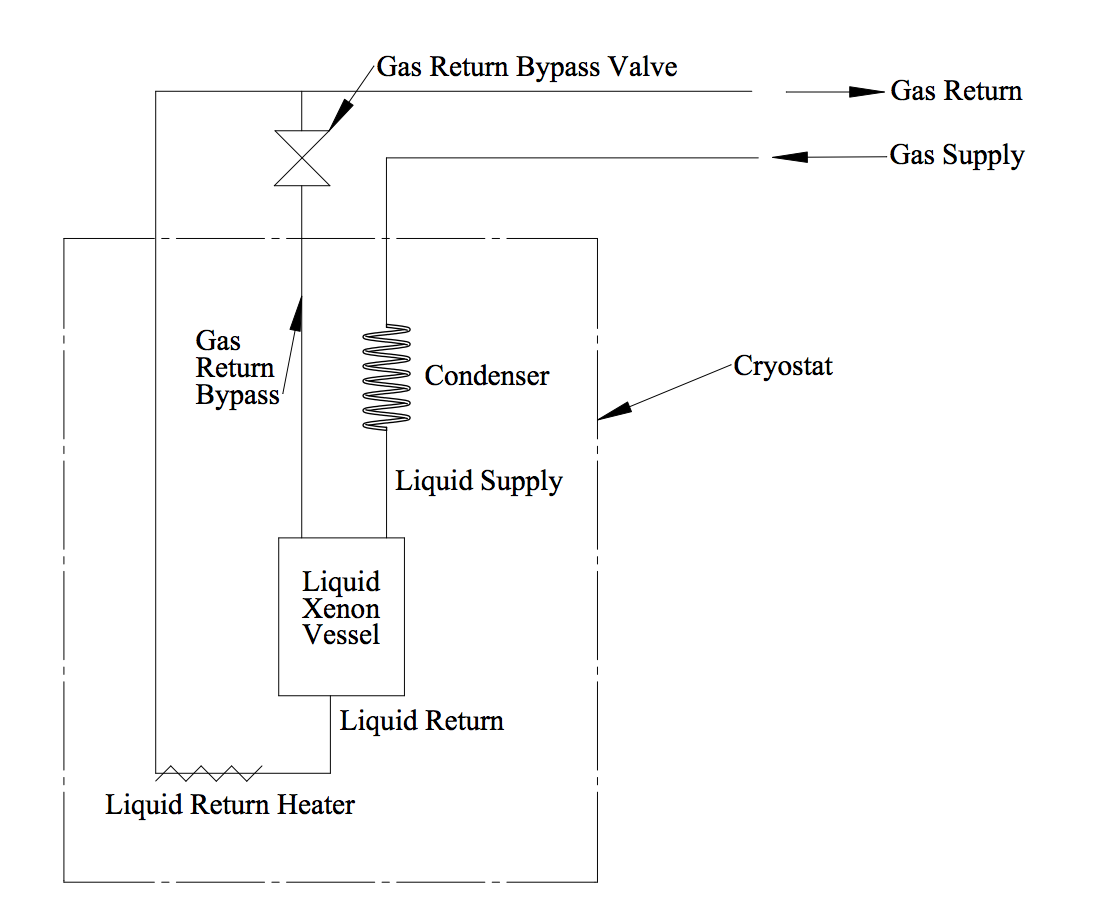
\includegraphics[scale=0.45]{img/CryoGas1.png}
	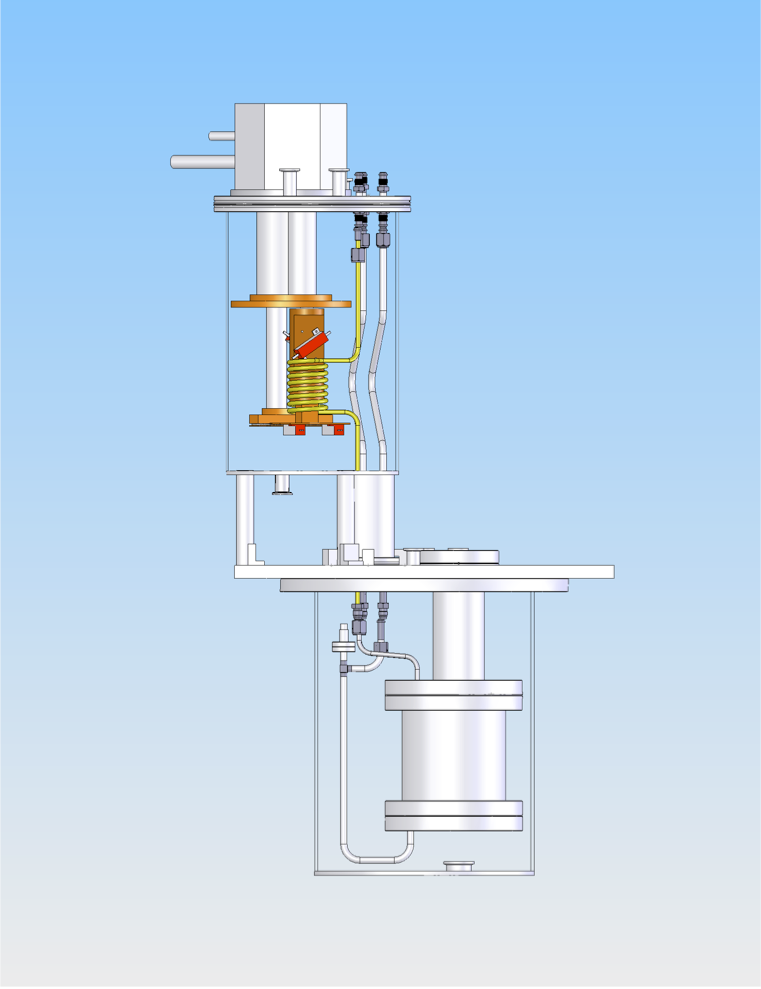
\includegraphics[scale=0.45]{img/CryoGas2.png}
	\caption{\label{fig.cryo} Left: P2 components. Right: a drawing of P2. The upper part of the cryostat holds the condenser, and the lower part holds the liquid xenon vessel (LXV). The P2 experiments will be carried out placing several setups inside the LXV.}
\end{figure}

\begin{figure}[!htb]
	\centering
	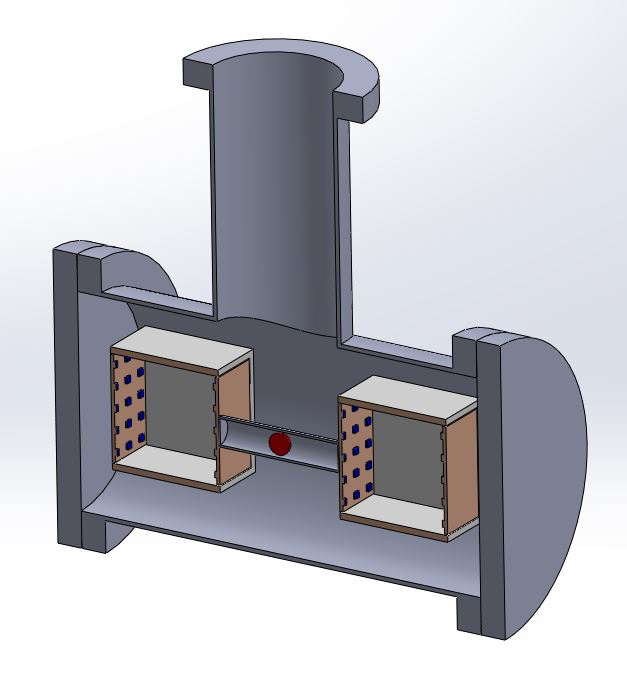
\includegraphics[scale=0.45]{img/P2.png}
	\caption{\label{fig.P2} A drawing showing the experimental arrangement in P2. The setup shows two LXSC2 with the radioactive source in a sealed container. }
\end{figure}

P2 is a general purpose apparatus suitable for studies of LXSC performance as well as other research activities. Figure \ref{fig.cryo}--left shows the components of the P2 setup. Room temperature gas flows to the condenser. Liquid drips into the liquid xenon vessel (LXV), and cool gas returns through the gas return line. The gas can also return through the liquid return line when no liquid is present. Figure \ref{fig.cryo}--right shows a drawing of P2. The upper part of the cryostat holds the condenser, and the lower part holds the LXV. The P2 experiments will be carried out placing several setups inside the LXV (figure \ref{fig.P2}). 

The construction of the P2 prototype involves three well defined tasks: 
\begin{enumerate}
\item {\bf Construction of the cooling system}, which includes the cryocooler, the condenser, the LXe vessel and the cryostats.  The system includes a vacuum pump to make vacuum in the LXe vessel before the liquid fill.
\item {\bf Construction of the gas system}, which includes the piping, recirculation pump and getter. The system includes an RGA to monitor the levels of impurities in the system. 
\item {\bf Construction of the experimental setups}. Two LXSC2 model A, and two LXSC2 model B will be 
manufactured:
\begin{itemize}
\item {\em Model A}, will be LXSC2 of $50 \times 50 \times 50 \mathrm{~mm^3}$, with two instrumented faces and all the others covered by reflective Teflon. Each instrumented face will deploy a matrix of $8 \times 8$~SiPMs of 6 mm length called Dice Board (DB). The SiPMs will be of conventional type, coated with TPB.
\item {\em Model B}, will be boxes of $25 \times 25 \times 50 \mathrm{~mm^3}$, with two instrumented faces and all the others covered by reflective Teflon. Each instrumented face will deploy a DB of $8 \times 8$~SiPMs of 3 mm length. The SiPMs will be VUV-sensitive (currently the maximum size of VUV sensitive SiPMs is 3 mm). 
\end{itemize}
\end{enumerate}

The three tasks can be carried out essentially in parallel, since most of the parts required are manufactured by industrial suppliers and can be ordered at the same time. The estimated time for the construction of P2 is 12 months. 

%A full-time mechanical engineer with expertise in cryogenics is needed for the design, assembly and commissioning of the system. The engineer will have the support of the IFIC engineering group and the support of the NEXT experiment, in particular concerning the construction and commissioning of the gas system (which will be a simplified version of the gas system built for the NEXT-DEMO detector, currently operating at IFIC). The estimated time needed to design, construct and commission P2 is one year. 

%Specifically, we will build two LXSC2 equipped with VUV-sensitive SiPMs (LXSC2-VUV) and two LXSC2 equipped with conventional SiPMs coated with TPB (LXSC2-TPB). The dimensions of the 
%\begin{enumerate}
%\item {\bf Yield}: the measurement of scintillation yield and time dependence in LXe will be done with a LXSC2 of 
%$25 \times 25 \times 25 \mathrm{~mm^3}$~equipped with 3 mm VUV-sensitive SiPMs. (LXSC2-VUV-1).
%\item {\bf Resolution}: 
 
%The first round of measurements can be done with a single LXSC, while the second round of measurements will be done with two LXSCs facing each other. A sealed tube (called the radioactive source holder, RSH), kept at a light vacuum will be placed in the middle of the two LXSC and will hold the radioactive Na-22 source for coincidence studies. The gammas within the angular acceptance of the RSH will exit the tube and enter the LXSCs through thin mylar windows. Gammas outside the acceptance will be attenuated by the LXe filling the vessel (and the LXSCs). 


\subsubsection*{Simulation and reconstruction}
While the P2 detector is being built, a full simulation toolkit, called SIMPLE will be developed. The toolkit, based in GEANT-4, will permit a full simulation of the P2 and PEP apparatus, as well as that of a future full-body PETALO 
scanner. SIMPLE is an essential tool to understand the response of the prototypes, as well as to prepare and test the imaging algorithms.

In parallel to SIMPLE a reconstruction and analysis framework (RAP) will be written. RAP will be tested on Monte Carlo data, so that it is available when P2 starts operation. 

%Based on SIMPLE and RAP, algorithms for imaging (calculation of LORs, filtered backprojection , TOF algorithms, maximum Likelihood expectation methods and machine learning methods) will be prepared. 

SIMPLE and RAP will be developed in parallel with P2 construction (12 months).  

\subsubsection*{Operation of the P2 prototype}
The operation of P2 will address objectives 1-4 of the project. P2 will be operated during a period of 12 months, in parallel with the construction of PEP. The operation of P2 will be coordinated by the DET subproject, but personnel from the other two subprojects as well as from the CLUES  project will participate in the experiments and data analysis. 

%permit a number of measurements, essential to understand the performance of LXe and its potential for medical imaging. Specifically, P2 will provide:
%\begin{enumerate}
%\item A precise measurement of the yield of 511 keV photons and its time dependence, two crucial parameters for PET performance which are still today affected of considerable systematic uncertainties.
%\item A systematic measurement of the performance of the LXSC (including energy resolution, spatial resolution and CRT). 
%\item A systematic measurement of the performance of different SiPM in LXe. We will study the dependence of the time resolution with the SiPM capacitance, the reduction of dark current, and measure the CRT that can be achieved with VUV--sensitive SiPMs and with SiPMs coated with TPB. 
%\item A systematic evaluation of state-of-the-art custom ASIC electronics for TOF-PET. Specifically we will study the performance of the TOF PET ASIC from PETSYS \footnote{http://www.petsyselectronics.com/web/public/products/1}. 
%\item We also intent to collaborate with a group of researchers from UB \footnote{PI D. Gasc\'on, henceforth UBG} to evaluate other alternatives, such as FlexToT \footcite{Trenado:2014vba}. 
%\item We will study the eventual operation of PETSYS and/or FlexToT electronics in LXe cryogenic conditions.
%\item In collaboration with the UBG, we will study the performance of fast detectors (such as MCPs or SPADs) with fast custom electronics (provided by the UBG) with the aim of detecting and exploiting for CRT measurements the Cherenkov light produced in xenon.  
%\end{enumerate}
%
%The operation of P2 and the analysis of the P2 data will extend over 18 months, in parallel with the construction of the larger PEP prototype. The operation of P2 requires from the DET subproject a post-doc fully dedicated to perform the experiments needed to study the various parameters and analyse the data. This project is also ideal for a graduate student. The post-doc and the student will work under the direct supervision of the PI. The operation and analysis of P2 data will also benefit from the collaboration of the ASIC subgroup and the UBG (items 4 to 6).

\subsubsection*{Construction and initial commissioning of the PEP prototype}

\begin{figure}[!htb]
	\centering
	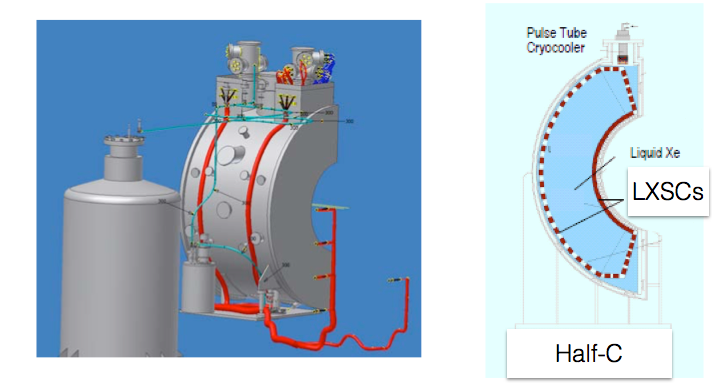
\includegraphics[scale=0.45]{img/HalfC.png}
	\caption{\label{fig.halfC} The half-C cryostat concept pioneer by the MEG experiment can be applied directly
	to PEP and a future large-scale PETALO scanner. }
\end{figure}

Figure \ref{fig.halfC} shows the half-C cryostat concept pioneer by the MEG experiment, which can be applied directly to PEP and a future large-scale PETALO scanner. The detector combines two half-C's in which the entry
faces are thin steel sheets (about 0.4 mm thick), while the rest of the container is reinforced to hold comfortably
	the pressure difference in the vacuum interfaces.  The cryocooler is directly coupled to the cryostat.    

The two half-C's of PEP will close to form a ring of inner diameter 230 mm, which will host 14-LXSCs
of dimensions  $50 \times 50 \time 25\mathrm{~mm^3}$~read out by a single DB type A(an $8 \times 8$~matrix made of 6-mm, blue sensitive SiPMs coated with TPB). PEP implements one layer of SiPMs, rather than two, to reduce costs. The thickness of the LXe cell is reduced accordingly to half of the nominal thickness of the LXSC2. 

The construction of PEP will take 12 months. The DET subproject will be in charge of the cryogenics, gas system and mechanics of the LXSC assembly, while the ASIC subproject will be in charge of the instrumentation and electronics of the LXSCs. 

%The construction of PEP requires a full-time engineer for 18 months.  


\subsubsection*{Operation of PEP}
PEP will be operated for a period of 6 months at IFIC and will be installed at the hospital LaFe during the last 6 months. The DET group has the responsibility to guarantee correct operation an maintenance of the apparatus. The IMG group has the responsibility of integrating PEP in a clinical environment. 

The initial operation of PEP will allow to measure the technical parameters of the scanner (resolution, sensitivity, CRT, etc.). Operation at the hospital LaFe will focus in the reconstruction of images and the extraction of biomarkers. 

%The post-doc assigned to software in the DET group, as well as the graduate student will participate in the imaging studies that will be led by the IMG group once the detector is fully operational. 

